\section{State of the art}

\subsection{Plant as sensor}

\subsubsection{Human-Plant cohabitation}

Plants have a lot of benefic effects on human. The study from Charles Hall and Melinda Knuth \cite{hallUpdateLiteratureSupporting2019}
explain all the benefits of plants on our human system.
Watts and al. shows that urban "greening" (add green spaces in urban city)
increase tranquility, relieve stress and anxiety \cite{wattsEffectsGreeningUrban2017}.
An experience has been conducted in offices by Ikei and al \cite{ikeiPhysiologicalPsychologicalRelaxing2014}
to expose roses to employees. The experience showed that the "parasympathetic nervous activity was significantly higher while viewing the rose". The subjects were more comfortable
being expose to roses than people that were not.
% Make plants the perfect interface, not harmful, enhance the link

\subsubsection{Human-Plant interaction}

The human plant interaction has been studied. Seow and al. \cite{seowPudicaFrameworkDesigning2022}
created a framework that is able to detect when something (and someone) interact with a plant.
However, this is not any plant, the plant used is the \textit{Mimosa Pudica}. This plant is special,
when something touches its leaves, the plant closes its leaves to protect them from the danger \cite{volkovMimosaPudicaElectrical2010}. 
An electrical impulse is released and is catch by the device Seow and al. developed. The electrical 
signal is easy to catch and thus can be used as actuator. However, the plant needs time and energy
to re-open the leaves. This framework also can't be generalized to other species of plants.

\begin{figure}[h!]
    \centering
    \includegraphics[width=0.8\textwidth]{pudica_framework.png}
    \caption{\textit{Pudica framework} made by Seow and al. The \textit{Mimosa Pudica} is a
    special plant that react to the interaction by closing its leaves. The framework
    captures the electrical impulse and then interprets that an interaction happened.} 
    \vspace{0.1cm}
    \label{fig:pudica_framework}
\end{figure}

Sato and al. used the process of capacitive sensing to detect interaction with objects of our daily lives \cite{satoToucheEnhancingTouch2012}.
In this paper, they proposed a device called \textit{Touché} that use swept frequency capacitive sensing  to detect touch interaction 
but also more complex interactions (such as interacting with a finger, the whole hand...). More complex 
interactions are captured using machine learning algorithm.

This paper doesn't apply the device to plants. Poupyrev and al. \cite{poupyrevBotanicusInteracticusInteractive2012}
used the device on plant to demonstrate the usage. This swept frequency technique is usable and better
than the previous single frequency technique as it captures more data.
In their article, Honigman and al. \cite{honigmanTechniquesSweptFrequencyb} adapted the \textit{Touché}
device to be use with an Arduino\footnote{Open source compute unit} microcontroller. This allowing people
to reproduce the set-up easily.


\subsubsection{Plant as sensors Plant transformed into sensors}

\subsubsection{Touch sensors}

Usual sensors uses physical properties to capture the data. For instance, in 1999, Hinckley and al. \cite{hinckleyTouchsensingInputDevices1999} 
were building a touch sensor made of conductive paint. The conductive paint is used as an electrode.
In the circuit, a component is generating a 30 Hertz square signal. When the user interact with the conductive surface,
it shifts and induce delay in the square wave. The delay induce by the user hands is caused by its natural
capacitance. This circuit, however, gives a boolean output based on a threshold. The answer is \textit{touched}
or \textit{untouched}. % Evoke the "The present work has demonstrated that touch-sensing is an
% orthogonal property of input devices that does not
% necessarily have to be coupled with position sensing

When thinking of touch sensors, we think about the trackpad/touchpad that we daily use in our personal 
computer. Those sensors use resistive or capacitive sensing. Both of these techniques are based on electrical
properties. Resistive sensing is based on the perturbation of the resistance in a circuit. Whereas 
capacitive is based on the capacitance. Capturing those specific properties are usually the basic of 
touch sensors.

For instance, Olberding and al. created a cuttable multitouch sensor based on capacitive sensor \cite{olberdingCuttableMultitouchSensor2013}.
This specific sensor allows to create something similar to a trackpad but with different shapes.

Reading the capacitance at a fixed frequency is working and is already used in our daily lives. 
However, to capture more complex interaction and to rely on the data, adding another dimension of data is useful.
Swept Frequency Capacitive sensing consists on emitting a electrical signal and then read the capacitive values
similar to what a classic sensor would do. However, the electrical signal is not generated at a fix frequency
but is generated following a changing frequency. 
Sato and al. introduced first this technique in the \texit{touché} device \cite{satoToucheEnhancingTouch2012}.
This allows to get richer information on the output of the device. \textit{Touché} allows then to capture 
the information on a variety and a multitude of daily objects.
Indeed, searching through many frequencies make it simpler to find small changes and though different kind and type 
of interactions.

\subsubsection{Sonification}

Sonification is “the use of non-speech audio to convey information or perceptualize data” \cite{hermannListenYourData}.
Herman and al \cite{hermannListenYourData} created two sonification models to represent particles moving. They are 
saying that the sonification is allowing a multidimensional representation of the data captured.
Humans are sensible to sounds. The sound allows a "rapid screening" because it is easier to listen to a sound than
read a graph or a text. The sound when combined with visualization is bringing more granularity and understanding.
They are also adding that we are using sound to diagnosis issues on a daily basis ; giving the example of a car
mechanic that is having a failure and that we can predict.


\subsubsection{Sonification on microcontrollers}

MCUs\footnote{microcontrollers} \cite{rochim2019design} is a kind of small computer.
Those devices can be used to generate sound. The most common way of doing electronical music
is to use MIDI\footnote{Musical Instrument Digital Interface} \cite{loyMusiciansMakeStandard1985}.
MIDI has been created in order to create music with digital computer. MIDI do not describe directly 
the audio signal but the human actions to create the signal (such as turn the knob left, push the slider...).
MCU are able to produce those kind of directives \cite{fazendaProceedingsInternationalConference1}\cite{fazendaProceedingsInternationalConference2}.
However, the MCU can produce MIDI but MIDI does not directly generate sounds. A synthetizer is needed to create the sound
described.

For our use case of embedding the device, we look at MCU that were able to directly generate the signal 
from a DAC\footnote{Digital to Analog Converter}. Projects had been conducted with many microcontrollers such as a small
8 bits AVR microcontrollers (ATmega32) \cite{hussainAVRMicrocontrollerImplementation2011}. This paper does not include limitation of
such a product but we can guess that the 8 bits microcontroller is limiting the sound quality. A larger project from Shaer and al.
\cite{shaerInteractiveCapacitiveTouch2020} is including an Arduino Mega controlling the visual effect of the project,
but also the interaction sensors. The Arduino Mega is then sending MIDI information to Teensy 3.2. The Teensy is then 
generating the sound. The project is still too large to be fully embedded but the Teensy 3.2 is a promising compute unit.
The Teensy 3.2 is running at 72 MHz, way faster than the ATmega32 that is operating at 16MHz. The frequency is essential
when trying the produce sound signals.


\subsubsection{Commercial products}

Generating music from plants is not a new concept. Several commercial products are available on the market.
Looking at \textit{PlantWave} device from the eponym company, the device is able to generate sound from the plant. The device is
built using a small box with two electrodes. The electrodes are then connected to the plant. The device generates sound.
The process of sonification is not described and thus is blurry as it is a patent technology. The device is also not open-source

\begin{figure}[h!]
    \centering
    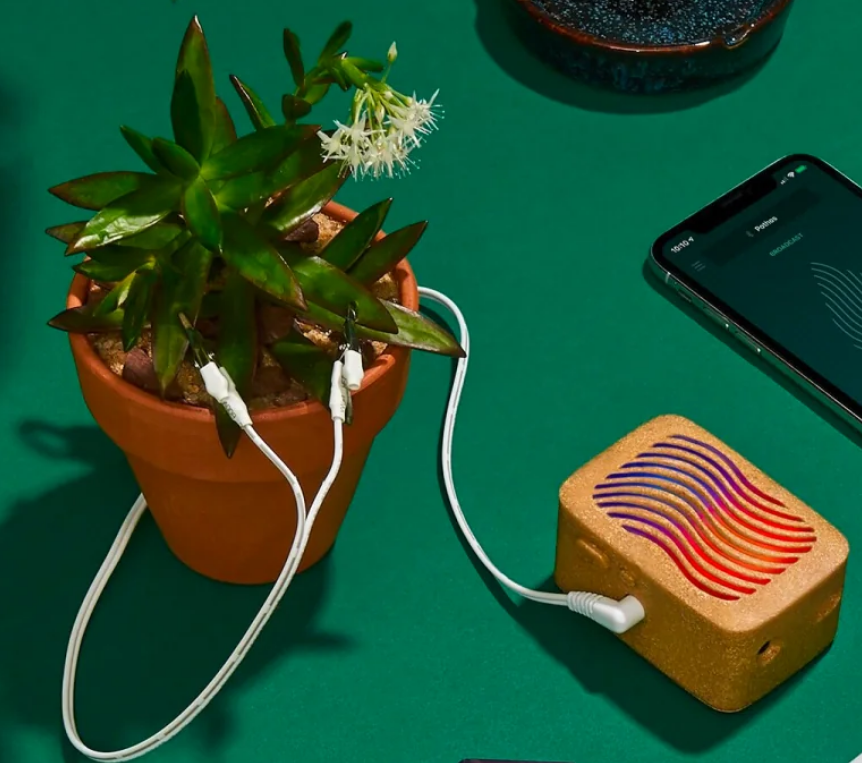
\includegraphics[width=0.8\textwidth]{images/plant_wave_product.png}
    \caption{The PlantWave product on a demonstration picture (source from their website)} 
    \vspace{0.1cm}
    \label{fig:plant_wave_product}
\end{figure}

Another commercial product is the \textit{Music of the Plants} product. How the product works is even more opaque and the company building the product
is sometimes associated with cult and esotericism. The product is also not open-source.


\subsection{Internet of Plants}

The Internet of Plants in not a new word. Nevertheless, the term is not that spread around.
Aliev and al. \cite{alievInternetPlantsApplication2018} evoked the word. The paper explain that
the word is based on the IoT\footnote{Internet of Things}. The paper is using this word 
to describe a system of sensors to monitor plants and crops. This is really close to the IoT
as it is using silicon made sensor to retrieve the data from the plants.

Internet of Plants is especially used for agriculture. In the paper of Steeneken and al.
\cite{steenekenSensorsAgricultureInternet2023}, they are explaining that the use of specific
sensors could and should be very efficient to boost the productivity of the crops.
The paper is also using talking about classic connected sensors but applied to plants.

Like the previous authors, Kitano and al. \cite{kitanoInternetPlantsIoP2022} also used 
this specific word for sensor connected agriculture. I think that the IoP of plants in 
that use is more a specific application of the IoT instead of a specific field of research.


\subsubsection{Distributed instruments}



\subsubsection{Sonification using software}